\documentclass[a4paper, 12pt]{article}
\usepackage[ngerman]{babel}
\usepackage[utf8]{inputenc}
\usepackage{amsmath}
\usepackage{amsfonts}
\usepackage{listings}
\usepackage{pgfplots}
\usepackage{graphicx}
\pgfplotsset{compat=1.9}
\usepackage{tikz}
\usepackage{float}


\author{Autor \\ Lukas Hofmaier \and Betreuer\\ Prof. Hansjörg Huser \\}
\title{Recommender System basierend auf Haskell \\ \vspace{2 mm} {\large Ein Report zu User-based Collaborative Filtering und Matrixfaktorisierung}}

\date{
\textsc{University of Applied Science Rapperswil}\\
Projektarbeit \\ \today
}

\begin{document}

\lstset{basicstyle=\small,
language=Haskell,
stringstyle=ttfamiliy
}

\clearpage\maketitle
\thispagestyle{empty}
\newpage
\setcounter{page}{1}
\tableofcontents
\newpage

\begin{abstract}
Recommender nutzen Datenbanken mit Präferenzen von Kunden, um ihnen aus einer grossen Auswahl von Artikeln diejenigen zu empfehlen, die sie interessieren könnten. Collaborative Filtering ist eine Klasse von Recommender, die Empfehlungen aufgrund von Verhaltensmuster anderer User berechnen.
In diesem Report werden zwei Collaborative Filtering Methoden beschrieben. User-based Collaborative Filtering ist eine der ersten und einfachsten Methoden. Matrixfaktorisierung ist eine weitere Methode, die an der Netflix Competition die besten Resultate lieferte.

Die Algorithmen werden mit einer geeigneten Evaluation verglichen. Die Evaluation und die Algorithmen wurden in Haskell implementiert.

\end{abstract}

\section{Recommender-Problem}
\label{sec:problem}

Konsumenten werden heute in vielen Bereichen mit einer unüberschaubaren Anzahl an Kaufmöglichkeiten konfrontiert. In einem Webshop für Bücher oder Filme ist es für den Konsumenten beispielsweise schwierig, alle Artikel im Angebot anzuschauen und aufgrund dieser Evaluation die besten Artikel auszuwählen. Beim Recommender-Problem geht es darum aus einer Menge von Artikeln (Items) eine sortierte Liste mit den empfehlenswerten Artikeln für einen spezifischen Kunden (User) zu erstellen. Recommender kommen vor allem dort zum Einsatz, wo persönlicher Geschmack bei der Bewertung von Artikeln eine wichtige Rolle spielt.

Ein Recommender kann eine Bewertung abschätzen (vorhersagen), die ein bestimmter User einem bestimmten Item gibt. Recommender berechnen die Bewertungen für Items, die der User noch nicht gesehen hat. Die Items mit den besten Bewertungen werden dem User empfohlen.

Recommender werden vor allem im e-Commerce eingesetzt. Man kann sie aber auch dazu verwenden, um unwichtige Informationen von wichtigen zu trennen. Recommender können beispielsweise auch für Information Retrieval eingesetzt werden. Sie generieren eine Liste von Dokumenten die der User noch nicht gesehen hat \cite{herlocker00}.

In nachfolgenden Text wird hauptsächlich von User und Items gesprochen. Sie sind folgendermassen definiert.

\begin{description}
\item[User] User sind die Konsumenten. Für sie berechnet das Recommender System Empfehlungen. 
User haben Präferenzen und bewerten Items aufgrund des persönlichen Geschmacks. In einer Information Retrieval Anwendung können User auch einfach die Benutzer der Software sein.
\item[Item] 
Items können Artikel, Filme, Bücher, Dokumente etc. sein. Items werden den Usern empfohlen.
\end{description}

Der aktive User bezeichnet den User, für den Empfehlungen erstellt werden \cite{jannach11}.

Es gibt zwei unterschiedliche Strategien für Recommender: Content-based Filtering und Collaborative Filtering. Dieser Report beschäftigt sich hauptsächlich mit Collaborative Filtering. 

\subsection{Content-based Filtering}
\label{sec:contentbased}

Bei Content-based Filtering wird zu jedem Artikel und zu jedem User ein Profil erstellt. Dieses Profil enthält Informationen über die Eigenschaften von User und Item. Beispielsweise könnte man alle angebotenen Filme nach ihrer Genrezugehörigkeit bewerten. Ein Film kann einen Action und einen Romantikanteil haben. User können angeben, ob sie lieber Action oder Romantik mögen. Content-based Filtering sucht dann Filme, die am besten mit dem Profil des aktiven Users übereinstimmen. Eine Schwierigkeit an Content-based Filtering ist das Erfassen von Daten zu jedem Item und zu jedem User. Der User gibt seine Präferenzen oft selber ein, was den meisten aber zu mühsam ist.

\subsection{Collaborative Filtering}
\label{sec:collaborativefiltering}

Bei Collaborative Filtering wird das Verhalten von Usern in der Vergangenheit analysiert. Der Inhalt der Artikel ist egal. Da diese Strategie unabhängig vom Inhalt ist, kann sie für unterschiedliche Anwendungen eingesetzt werden. Es wird im e-Commerce sowie auch im Information Retrieval erfolgreich eingesetzt \cite{sarwar01}. 

Bei Collaborative Filtering geht man davon aus, dass sich User, die sich in der Vergangenheit für ein Item interessiert haben, auch in Zukunft dafür interessieren. 

Ziel des Collaborative Filtering ist, es das Interesse eines User an einem Item, das er noch nicht gesehen hat, automatisch vorauszusagen. Zu diesem Zweck werden Daten in Form von Bewertungen und Transaktionen gesammelt. Mithilfe dieser Daten wird nach Usern mit einem ähnlichen Verhaltensmuster gesucht. Die Vorhersage leitet sich von den Bewertungen der ähnlichen User ab. 

\subsubsection{Abgrenzung zu Content-based Filtering}
\label{sec:definitioncf}

Bei Collaborative Filtering werden die Bewertungen anderer User dazu benutzt, um dem aktiven User ein Item zu empfehlen, das er noch nicht gesehen hat. Im Unterschied zu Content-based Filtering ist der Inhalt des Items für die Empfehlung nicht relevant. Das einzige was zählt sind die Bewertungen anderer User.

\subsubsection{Vorteile}
\label{sec:advandage}
Gegenüber Content-based Filtering bietet Collaborative Filtering folgende Vorteile.

\begin{description}
\item[Kein Wissen über Inhalt nötig] Es muss nicht jedes Item nach seinem Content durchsucht werden. Meistens ist der Inhalt im Kontext der Empfehlung nicht relevant (Länge, Kategorie, Jahr).
\item[Usergeschmack ändert sich] Collaborativ Filtering passt sich automatisch an.
\item[Intuitiv] Jeder versteht "`Kunden, die diesen Artikel gekauft haben, haben auch diese Artikel gekauft"'.
\end{description}

\subsubsection{Nachteile}
 \begin{description}
\item[Rechnen mit dünn besetzten Matrizen] Für die Berechnung der Empfehlungen werden die Bewertungen zum Teil als Matrix abgespeichert. Die Zeilen repräsentieren Items und die Spalten User. Diese Item-User Matrix ist normalerweise sehr gross (ca. $10^{7}$ User, ca. $~10^6$ Items) und dünn besetzt. Darüber hinaus sind Rechenoperationen mit einer solchem Matrix sehr aufwändig.  
\item[Shilling Attacke] Wenn die User Items explizit bewerten können, besteht die Gefahr sogenannter Shilling Attacken. User haben die Möglichkeit Items unabhängig ihrer persönlichen Präferenz, gut oder schlecht zu bewerten. Dadurch steigt die Wahrscheinlichkeit, dass diese Items fälschlicherweise anderen User empfohlen werden.
\end{description}

\subsubsection{Resultate von Collaborative Filtering}
\label{sec:output}

Die Collaborative Filtering Algorithmen nehmen bestehende Bewertungen und ein User-Item Tupel $(u,i)$ als Argument und liefern eine Vorhersage $p_{u,i}$ für eine Bewertung.  $p_{u,i}$ drückt die Wahrscheinlichkeit aus, dass Item $i$ für User $u$ interessant ist. 

Meistens möchte man für einen aktiven User $u$ eine Liste mit $N$ Items, die ihn interessieren könnten und die er noch nicht gesehen hat. Um diese Liste zu erstellen, berechnet der Recommender für alle Items die Vorhersagen $p_{u,i}$ für den aktiven User $u$ und stellt eine Liste mit $N$ Items mit den höchsten $p_{u,i}$-Werten zusammen. Diese Liste nennt man Top-N Empfehlung. Abbildung \ref{fig:cfprocess} zeigt die beiden Resultate eines Recommender Algorithmus.

\begin{figure}
  \centering
      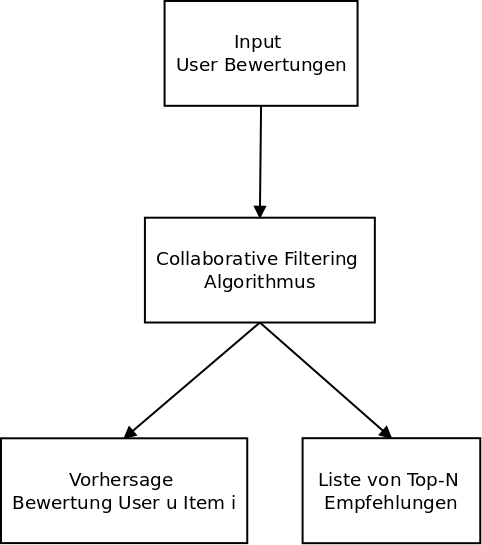
\includegraphics[width=0.5\textwidth]{cf}
  \caption{Collaborative Filtering Prozess}
  \label{fig:cfprocess}
\end{figure}

\subsubsection{Speicherbasiert Methoden vs. modellbasiert}
\label{sec:cfmodels}

Collaborative Filtering wird weiter in zwei unterschiedliche Methoden aufgeteilt:

\begin{description}
\item[Speicherbasiert] Bei speicherbasierten Methoden werden für jeden User ähnliche User aufgrund der gespeicherten Bewertungen gesucht. Es wird eine Nachbarschaft mit ähnlichen User erstellt. Diese Methoden nennt man auch Nächste-Nachbarn oder kNN-Methoden.
Ähnlichkeit wird aufgrund von gemeinsam bewerteten Items berechnet. Wenn zwei User für mehrere Items die selben Bewertungen vergeben, sind sie sich ähnlich. Sie haben einen ähnlichen Geschmack. Einem User werden diejenigen Items empfohlen, die er noch nicht kennt und die eine hohe Bewertung von ähnlichen Usern erhalten haben.
Wenn das Recommendersystem $p_{u,i}$ berechnen soll, beschafft es sich eine Liste mit allen Usern, die in der Nachbarschaft von $u$ sind und die das Item $i$ bewertet haben. Aufgrund der Ähnlickeit zu $u$ und den vorhandenen Bewertungen der User in der Liste für $i$, wird $p_{u,i}$ berechnet.
\item[Modellbasiert] Modellbasierte Methoden (englisch: model-based) nutzen die bestehenden Bewertungen um ein Modell zu erlernen. User und Items werden mit Vektoren repräsentiert. Die Elemente der Vektoren sind Präferenzen und Eigenschaften.  $p_{u,i}$ wird aufgrund dieser Vektoren berechnet. Die Berechnung des Modells kann auf ein Optimierungsproblem reduziert werden.
\end{description}

Dieser Report beschreibt Algorithmen für beide Methoden. User-based CF ist speicherbasiert. Matrixfaktorisierung ist modellbasiert.

\subsection{Herausforderungen}
\label{sec:challenges}

Bei der Implementierung von Recommendersystemen ergeben sich mehrere Herausforderungen.

\begin{description}
\item[Genauigkeit]  Die Differenz zwischen $p_{u,i}$ und der tatsächlichen Bewertung soll möglichst klein sein.
\item[Skalierbarkeit] 
Collaborative Filtering muss für Millionen User und Items möglich sein. Die Technik soll also für grosse Datenmengen skalieren.
\item[Dünn besetzte Matrizen] Für eine grosse Menge an Items gibt es in der Regel nur eine kleine Anzahl an Items, die ein User auch bewertet hat. Wenn sich keine gemeinsamen Items zwischen den Usern finden, können auch keine Nachbarschaften gebildet werden.
\end{description}

\section{Evaluation}
\label{sec:evaluation}

Dieser Abschnitt beschreibt eine Methode, um die Qualität der beschriebenen Recommender zu evaluieren. In den nachfolgenden Abschnitten werden die Algorithmen mit dieser Methode evaluiert und verglichen.

\subsection{Daten}
\label{sec:data}

Ein Recommenderalgorithmus benötigt Daten, um das Modell oder die Nachbarschaften zu erstellen. Für die Evaluation sind ebenfalls vorhandene Bewertungen notwendig.

Die Daten für Recommender Systeme können auf zwei unterschiedliche Arten beschafft werden.

\begin{description}
\item[Explizites Feedback] Bei explizitem Feedback verlässt man sich auf Daten, die User explizit eingegeben haben. Beispielsweise werden User aufgefordert, dem System ihre Präferenzen anzugeben oder man präsentiert den User eine Reihe von Items, die sie auf einer Skala von 1 bis 5 bewerten. 
\item[Implizites Feedback] Implizites Feedback leitet die Bewertungen der User für Items aus Beobachtungen ab. Das System beobachtet die Interaktionen, wie zum Beispiel in Vergangenheit gekaufte Artikel, Browsehistory, Suchanfragen oder Klickverhalten, des User mit dem System.
\end{description}

\subsubsection{MovieLens Daten}
\label{sec:movielens}

Für das Projekt wurden die Daten von MovieLens verwendet. MovieLens ist ein Recommender der vom GroupLens Projekt an der Universität Minnesota entwickelt wurde. Die Daten werden mit einer Webapplikation gesammelt. User können Filme bewerten und MovieLens gibt den User darauf eine Top-N Empfehlungsliste. Das heisst, die Daten wurden durch explizites Feedback gesammelt. Die Daten können von http://www.grouplens.org/node/12 heruntergeladen werden. 

Das Datenset enthält die Bewertung von 943 User und 1682 Items. Die Daten sind in Kolonnen strukturiert. Die erste und zweite Kolonne enthält User und Item ID. Die dritte Kolonne enthält ein Zahl zwischen 1 und 5. Sie repräsentiert die Bewertung. Und in der vierten Kolonne ist ein Zeitstempel der Bewertung. Das Movielens Datenset enthält insgesamt 100000 Bewertungen. Abbildlung \ref{fig:movielens} zeigt einen Auschnitt der rohen Daten.

\begin{figure}
\centering
\begin{verbatim}
1	1	5	874965758
1	2	3	876893171
1	3	4	878542960
1	4	3	876893119
1	5	3	889751712
\end{verbatim}
\caption{Ausschnitt aus MovieLens Datensatz}
\label{fig:movielens}
\end{figure}

Für den User-based Collaborative Filtering Algorithmus wurden die Daten mittels Python-Skript \verb|tocsv| in das CSV-Format transfomiert. Das CSV-Format eignet sich besser, weil vorhandene Softwarebibliotheken für das Einlesen der Daten genutzt werden können. In diesem Projekt wurden die Daten mit Paket \verb|cassava| eingelesen.

Für die Matrixfaktorisierung wurden die Daten als Matrix abgespeichert. So muss das Programm nicht bei jedem Testlauf die Transformation von 100000 Bewertungen in eine Ratingmatrix vornehmen.

\subsection{Vorgehen}
\label{sec:procedure}

Die Qualität der beschriebenen Recommender-Algorithmen wird durch die Genauigkeit der Bewertungsvorhersagen bestimmt. Man misst die Differenz zwischen vorhergesagter Bewertung $p_{u,i}$ und tatsächlicher Bewertung $q_{u,i}$. 
Um die Vorhersagen zu berechnen, muss man zuerst ein Modell aufgrund vorhandener Daten erstellen (Training). Danach werden mit diesem Modell Vorhersagen berechnet und mit den richtigen Bewertungen verglichen (Test). 

Die vorhandenen Daten werden entsprechend in ein Trainings- und Testset aufteilt. In diesem Projekt wurden die MovieLens-Daten in 80000 Bewertungen für die Trainingsphase und 20000 Bewertungen für die Testphase aufgeteilt.

Die Evaluation wird in zwei Phasen aufgeteilt. 

\begin{enumerate}
\item Trainingsphase
\item Testphase
\end{enumerate}

\subsubsection{Trainingsphase}

In der Trainingsphase wird ein Modell mithilfe des Trainingsset berechnet. Die Funktion \verb|model| nimmt als Argument das Trainingsset und gibt als Wert ein Modell zurück. Dieses Modell wird in der Testsphase der \verb|predict|-Funktion als Argument übergeben. 

Bei User-based Collaborative Filtering ist das Modell die Nachbarschaft jedes User. Bei Matrixfaktorisierung sind die erlernten Präferenzen und Eigenschaften der User und Items das Modell.

\subsubsection{Testphase}
In der Testphase wird für alle User-Item-Paare aus dem Testset die Vorhersage $p$ mit der Funktion \verb|predict| berechnet. Um die Genauigkeit zu bestimmen werden die Vorhersagen mit den tatsächlichen Bewertungen verglichen. 

\subsubsection{Evaluationsmetrik}
\label{sec:evaluationmetrik}

Um die Qualität der Recommender zu quantifizieren, wird die absolute mittlere Abweichung als Evaluationsmetrik verwendet. Nachfolgend wird diese Metrik mit MAE (engl. mean absolute error) bezeichnet. MAE wird für die Evaluation von Recommender häufig verwendet \cite{sarwar01}. 

Der MAE berechnet sich wie folgt: Für alle $N$ Vorhersagen $p$, die in der Testphase berechnet wurden, wird die Differenz zur tatsächlichen Bewertung $q$ berechnet. Die Abweichungen vom tatsächlichen Wert sind die Residuen. Von der Differenz wird der Betrag berechnet. Alle Abweichungen werden summiert. Schliesslich wird die mittlere Abweichung bestimmt, indem durch Anzahl Bewertungen $N$ im Testset geteilt wird. 

\begin{equation}
  \label{eq:mae}
  MAE = \frac{\sum_{i+1}^N | p_i-q_i | }{N}
\end{equation}

Abbildung \ref{fig:crossvalidation} stellt das Vorgehen der Evaluation grafisch dar.

\begin{figure}
  \centering
      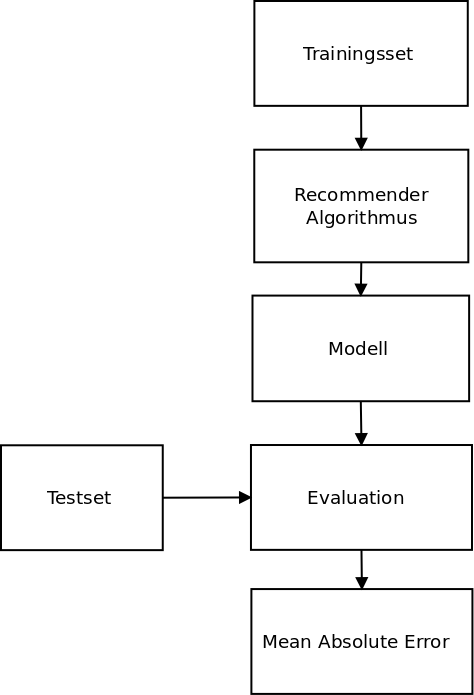
\includegraphics[width=0.5\textwidth]{evaluationn}
  \caption{Die Evaluation der Recommender}
  \label{fig:crossvalidation}
\end{figure}

\subsubsection{Implementierung}

Listing \ref{lst:mae} zeigt die Implementierung der Evaluation in Haskell. Die Funktion \verb|mae| nimmt als Argumente eine Funktion, die ein User-Item Tupel auf eine Vorhersage abbildet(die \verb|predict| Funktion), das Testset und gibt den MAE zur"uck. Die Funktion \verb|predict| wird partiell auf das Modell angewendet. Deshalb nimmt sie in der Funktion \verb|mae| nur noch einen User und ein Item.

\begin{lstlisting}[caption=Berechnung des MAE in Haskell , label=lst:mae]
mae :: (Int -> Int -> Double) -> Vector Rating -> Double
mae predict v=sum errors predict v/fromIntegral length v

errors :: ( User -> Item -> Double )
       -> Vector Rating
       -> Vector Double
errors predict v = map diff v
  where diff (u, i, r) = abs (r - predict u i)
\end{lstlisting}

\section{Unpersönliche Empfehlungstechniken}
\label{sec:simple}

Dieser Abschnitt beschreibt einfache, alternative, Möglichkeiten relative gute Empfehlungen zu generieren. Diese Techniken werden in den nachfolgenden Abschnitten als Baselinealgorithmus verwendet, um zu überprüfen, ob die beschriebenen Algorithmen einen tieferen MAE-Wert erreichen. So ist einfach ersichtlich, ob die Collaborative Filtering Algorithmen einen qualitativen Vorteil bringen.

Um einem User Items zu empfehlen werden oft einfache Statistiken berechnet. Diese Methoden sind unpersönlich. Das heisst die Top-N Empfehlungen sind nicht vom persönlichem Geschmack abhängig. Jeder User erhält die selben Empfehlungen. 

Diese Technik wird in vielen Bereichen angewendet. Restaurantführer oder Filmkritikwebseiten erstellen oft Ranglisten, welche Restaurants oder Filme von allen Usern im Durchschnitt am besten bewertet werden. Items mit den höchsten Durchschnittswerten, werden dem User empfohlen \cite{jannach11}.

Die einfachste Methode, eine unbekannte Bewertung $p_{u,i}$ abzuschätzen, ist den Durchschnitt aller Bewertungen zu berechnen.

\begin{equation}
  \label{eq:avg}
  p_{u,i} = \mu
\end{equation}

Wenn diese Methode evaluiert wird, erhält man einen MAE von 0.968. Dieser Wert kann noch weiter minimiert werden.

Bestimmte User vergeben durchschnittlich tiefere Bewertungen. Diese Tendenz $b_u$ kann für jeden User berechnet werden. Es wird die Abweichung der Bewertungen des Users $u$ vom Erwartungswert $\mu$ berechnet.

\begin{equation}
  b_u = \frac{1}{|I_u|}\sum_{i \in I_u}(r_{u,i} - \mu)
\end{equation}

Die Menge $I_u$ beinhaltet alle Items, die der User $u$ bewertet hat. $r_{u,i}$ ist die Bewertung die User $u$ Item $i$ gegeben hat.

Die Abweichung $b_u$ wird bei der Vorhersage zu $\mu$ addiert, um bei der Evaluation einen besseren MAE zu erhalten.

\begin{equation}
  \label{eq:bui}
  p_{u,i} = \mu + b_u
\end{equation}

Wenn man die Tendenz der User, Item durchschnittlich höher oder tiefer zu bewerten, berücksichtigt wie in der Gleichung \ref{eq:bui} beschrieben, kann man den MAE auf 0.8501 senken. 

Items haben ebenfalls eine Abweichung vom Durchschnitt. Bestimmte Filme können tendenziell eine höhere Bewertung von allen Usern erhalten. Es kann also noch die Abweichung $bi$ jedes Items berechnet werden.

\begin{equation}
  \label{eq:bi}
  b_i = \frac{1}{|U_i|}\sum_{u \in U_i}(r_{u,i} - b_u - \mu)
\end{equation}

Diese Abweichung addiert man zur Vorhersage $b_{ui}$.

\begin{equation}
  \label{eq:baseline}
  p_{u,i} = \mu + b_u + b_i
\end{equation}

Wenn man die statistischen Abweichungen der einzelnen User und Items bei der Vorhersage einer Bewertung $b_{ui}$ wie in Gleichung \ref{eq:baseline} berücksichtigt, erreicht man einen MAE von 0.76814.

$p_{ui}$ kann relativ einfach aufgrund der vergangen Bewertungen berechnet werden.

In Abbildung \ref{fig:maebaselines} werden die verschiedenen, unpersönlichen Recommender miteinander verglichen. 

\begin{figure}
  \centering
\begin{tikzpicture}
  \begin{axis}[
    xbar, xmin=0,
    width=12cm, enlarge y limits=0.5,
    symbolic y coords = {Globaler Durchschnitt,mit Usertendenz $b_u$, mit User-/Itemtendenz},
    xlabel={MeanAbsoluteError},
    ytick = data,
    nodes near coords, nodes near coords align={horizontal},
    ]
    \addplot coordinates {(0.968,Globaler Durchschnitt) (0.8501,mit Usertendenz $b_u$) (0.76814,mit User-/Itemtendenz)};
  \end{axis}
\end{tikzpicture}
  
  \caption{Vergleich: unpersönliche Empfehlungstechniken}
  \label{fig:maebaselines}
\end{figure}


\section{User-based Collaborative Filtering}

Die Technik User-based Collaborative Filtering (nachfolgend User-based CF) ist auch als k-NN (Nächste-Nachbarn) oder User-User Collaborative Filtering bekannt. Der GroupLens Usenet Artikel Recommender verwendete als einer der ersten Recommender Systeme User-based CF. Ringo Music Recommender und der Bell Core Video Recommender verwenden auch User-based CF \cite{ekstrand11}.

User-based CF sucht ähnliche User wie der aktive User und verwendet ihre Bewertungen für Item $i$ um $p_{u,i}$ zu berechnen.

\subsection{Informelles Beispiel}
\label{sec:example}

Die Wahrscheinlichkeit, dass der Film Titanic für User Peter interessant ist wird berechnet.
Der Recommender sucht nach anderen Usern, die Filme ähnlich bewerten wie Peter. Dazu beschafft er sich für jeden anderen User eine Liste aller Filme, die Peter und der andere User bewertet haben. So findet er heraus, welche User Peter am ähnlichsten sind. Das ist seine Nachbarschaft $N$. Um vorherzusagen, welche Bewertung Peter Titanic gibt, verwendet der Recommender die Bewertungen für Titanic der User in $N$. Wenn ähnliche User Titanic eine hohe Bewertung geben, wird eine hohe Bewertung von Peter vorhergesagt. Die Bewertung von Usern, die Peter sehr ähnlich sind, haben ein grösseres Gewicht als die Bewertungen von Usern, die Peter unähnlich sind.

\subsection{Ähnlichkeit bestimmen}
\label{sec:neigborhood}

Es gibt mehrere Methoden die Ähnlichkeit zwischen zwei Usern zu bestimmen.
Die Genauigkeit der Vorhersagen $p_{u,i}$ ist von der Wahl der Methode abhängig.
Dieser Abschnitt beschreibt die Definition und die Implementierung der Ähnlichkeit-Metrik Pearson-Korrelation.

\subsubsection{Pearson-Korrelation}
\label{sec:pearsoncorrelation}

Gemäss \cite{jannach11} eignet sich das Mass Pearson-Korrelation (auch Korrelationskoeffizient) gut für User-based CF. Es ist ein Mass für den lineare Zusammenhang von zwei Listen und nimmt Werte zwischen -1 und +1 an. +1 bedeutet, dass die Listen sehr ähnlich sind. -1 bedeutet dass sie unähnlich sind. Bei 0 besteht kein Zusammenhang.

Pearson-Korrelation berücksichtigt den Umstand, dass User Items konstant tiefer oder höher bewerten. Zwei User, die mit den Vektoren (1,2,3,4) und (2,3,4,5) dargestellt werden, erhalten die maximale Ähnlichkeit von 1.

Die Pearson Korrelation ist folgendermassen definiert.

\begin{equation}
\label{eq:pearson1}
 sim(u,u') = \frac{cov(X,Y)}{\sigma_X \sigma_Y} 
\end{equation}
oder
\begin{equation}
  \label{eq:pearson}
  sim(u,u')  = \frac{\sum_{i \in I_u \cap I_u'}(r_{u,i} - \bar{r}_u)(r_{u',i} - \bar{r}_{u'})}{\sqrt{\sum_{i \in I_u \cap I_{u'}}( r_{u',i} - \bar{r}_{u'})^2}\sqrt{\sum_{i \in I_u \cap I_{u'}}( r_{u',i} - \bar{r}_{u'})^2}}
\end{equation}

$I_u \cap I_{u'}$ ist die Liste aller Items, die User $u$ und User $u'$ bewertet haben. $r_{u,i}$ ist die Bewertung von User $u$ für Item $i$. 


Das Paket \verb|Math.Statistics| stellt die Funktion \verb|pearson| zur Verfügung um den Korrelationskoeffizenten zu berechnen.
\begin{verbatim}
pearson::Floating a => [a] -> [a] -> a
\end{verbatim}
 Der Funktion \verb|pearson| nimmt zwei Listen mit den Bewertungen der gemeinsamen Items als Argument.

Um $sim(u,u')$ zu berechnen, wird die Liste $I_u \cap I_{u'}$ auf die Bewertungen $r_{u,i}$ der User $u$ und $u'$ abgebildet und der Funktion \verb|pearson| übergeben. Listing \ref{lst:shareditems} zeigt, wie $I_u \cap I_v$ beschafft wird. Die Funktion \verb|shareditems| nimmt die Argumente User $u$ und $u'$ und eine Map (Dictionary), die User auf die bewerteten Items abbildet, entgegen.

\begin{lstlisting}[caption=Implementierung der Abfrage von $I_u \cap I_{u'}$, label=lst:shareditems]
import Data.MultiMap
shareditems :: User 
            -> User 
            -> Multimap User Item 
            -> [Items]
shareditems u1 u2 m = shared (lookup u1 m) (lookup u2 m)
  where shared l1 l2 = [x| x <- l1, y <- l2, x = y]
\end{lstlisting}

Listing \ref{lst:item2rating} zeigt wie Items auf Bewertungen abgebildet werden. 

\begin{lstlisting}[caption=Implementierung: Abbildung Items zu Bewertungen, label=lst:item2rating]
import Data.MultiMap
item2rating:: [Item] -> Multimap Item Double -> [Double]
item2rating is m = map (\i -> findWithDefault 0 i m) is
\end{lstlisting}

Bei der Verwendung der Pearson-Korrelation sind folgende Schwierigkeiten aufgetreten.

\begin{description}
\item[Hohe Ähnlichkeit bei wenig Items] Die Berechnung Pearson-Korrelation zwischen zwei Usern, die nur ein Item gemeinsam bewertet haben führt zu relativ hohen Ähnlichkeitswerten, obwohl zwei User, die nur ein gemeinsames Item haben eher unähnlich sind.
\item[Abweichung 0] Wenn die Bewertungen eines Users für alle gemeinsamen Items  $I_u \cap I_v$ gleich sind, führt das zu einer Standardabweichung $\sigma$ von 0.  Die Pearson-Korrelation ist nicht definiert, wenn $\sigma_x$ oder $\sigma_Y$ 0 ist und somit ist in diesem Fall die Ähnlichkeit nicht definiert.
\item[Nur ein gemeinsames Item] Wenn $I_u \cap I_v$ nur ein gemeinsames Item enthält ist die Standardabweichung $\sigma$ immer 0.
\item[keine gemeinsamen Items] Wenn es keine gemeinsamen Items gibt, kann keine Ähnlichkeit berechnet werden.
\end{description}

In einem ersten Versuch wurden, die oben genannten Probleme durch entsprechende Fallunterscheidung in der Implementierung abgefangen. Listing \ref{lst:similarity} zeigt die Implementierung.

\begin{lstlisting}[caption=Similarity, label=lst:similarity]
import Math.Statistics

similarity :: [Double] -> [Double] -> Double
similarity r1 r2
  | (length r1) < 2 = 0
  | (length r2) < 2 = 0
  | stddev r1 == 0.0 = 0
  | stddev r2 == 0.0 = 0
  | otherwise = MS.pearson r1 r2

\end{lstlisting}

Wenn die Standardabweichung $\sigma$ 0 ist, gibt die Funktion \verb|similarity| einen Ähnlichkeitswert von 0 zurück.

Diese Implementierung der Ähnlichkeit hat zu einem MAE von 0.830 geführt. Der unpersönlichen Recommender aus Abschnitt \ref{sec:simple} hat einen MAE von 0.768 erreicht. Die Implementierung ist verbesserungswürdig. 

\subsubsection{Optimierung der Pearson-Korrelation}
\label{sec:optpearson}

Ein Grund für die Probleme ist, dass die Pearson-Korrelation aus Gleichung \ref{eq:pearson} nur die Bewertungen der gemeinsamen Items  $I_u \cap I_v$ bei der Berechnung der Ähnlichkeit berücksichtigt. Um das Problem der undefinierten Standardabweichung $\sigma$ zu beheben, wurde der Erwartungswert $\bar{r_v}$ der gemeinsamen Bewertungen durch den Erwartungswert $b_u$ aller Bewertungen des Users $u$ (siehe Abschnitt \ref{sec:simple}, Gleichung \ref{eq:bi}) ersetzt. Statt mit der Formel

\begin{equation}
  \label{eq:naiv}
  \sigma = \sqrt{\sum_{i \in I_u \cap I_v}( r_{v,i} - \bar{r}_v)^2}
\end{equation}

wird die Standardabweichung wie folgt berechnet:

\begin{equation}
  \label{eq:naiv1}
  \sigma = \sqrt{\sum_{i \in I_u \cap I_v}( r_{v,i} - b_u)^2}
\end{equation}

In die Gleichung \ref{eq:pearson} eingesetzt, berechnet sich die Ähnlichkeit folgendermassen:

\begin{equation}
  \label{eq:advanced}
  sim(u,v)  = \frac{\sum_{i \in I_u \cap I_v}(r_{u,i} - b_u)(r_{v,i} - b_v)}{\sqrt{\sum_{i \in I_u \cap I_v}( r_{v,i} - b_u)^2}\sqrt{\sum_{i \in I_u \cap I_v}( r_{v,i} - b_v)^2}}
\end{equation}

Da statt der Standardabweichung $b_u$ verwendet wird, kann nicht mehr die \verb|pearson|-Funktion aus dem Statistik-Paket verwendet werden. Die Funktion \verb|pearson| wurde durch eine eigene Implementierung der Gleichung \ref{eq:advanced} ersetzt.

\begin{figure}
\begin{tikzpicture}
  \begin{axis}[
    xbar, xmin=0.7, xmax=0.95,
    height=5cm,width=10cm, enlarge y limits=0.5,
    symbolic y coords = {Pearson Korr.,Opt. Pearson Korr.},
    xlabel={Mean Absolute Error},
    ytick = data,
    nodes near coords, nodes near coords align={horizontal},
    ]
    \addplot coordinates { (0.831,Pearson Korr.) (0.718,Opt. Pearson Korr.)};
  \end{axis}
\end{tikzpicture}
\centering
\caption{Vergleich der angepassten Berechnung der Ähnlichkeit mit normaler Pearson-Korrelation}
\label{fig:comparesim1}
\end{figure}

Abbildung \ref{fig:comparesim1} zeigt, dass die Berechnung der Ähnlichkeit mit Formel \ref{eq:advanced} den kleineren Fehler bei der Evaluation ergibt.

\subsection{Unbekannte Bewertung $p_{u,i}$ berechnen}
\label{sec:compp}

Um die Vorhersage $p_{u,i}$ zu berechnen, wird zuerst eine Nachbarschaft $N$ zu User $u$ und Item $i$ erstellt. $N$ erfüllt folgende Anforderungen:

\begin{itemize}
  \item  $N$ enthält $k$ Elemente.
  \item   $N$ ist absteigend nach der Ähnlichkeit $sim(u,u')$ sortiert. $N$ enthält $k$ User mit der höchsten Ähnlichkeit $sim(u,u')$.
  \item  $N$ enthält nur User $u'$, die Item $i$ bewertet haben.
 \end{itemize} 

Um die Nachbarschaft $N$ zu erstellen, wird für User $u$ die Ähnlichkeit $sim(u,u')$ zu allen anderen User berechnet.

In Listing \ref{lst:neighborhood} wird gezeigt, wie die Abfrage von $N$ in Haskell implementiert wurde. Die Funktion \verb|neighborhood| nimmt neben dem User $u$ und dem Item $i$ noch eine natürliche Zahl $k$ als Argument. $k$ bestimmt die Grösse der Nachbarschaft $N$. Ausserdem nimmt die Funktion noch eine Map (Dictionary). Diese Map bildet User $u$ auf eine Liste von Ähnlichkeiten zu allen anderen Usern ab. Die Ähnlichkeiten werden benötigt, um die Nachbarschaft $N$ zu sortieren und später $p_{u,i}$ zu berechnen.

\begin{lstlisting}[caption=Abfrage der Nachbarschaft $N$ in Haskell, label=lst:neighborhood]
import Data.MultiMap
neihborhood :: User
            -> Item
            -> Int
            -> MultiMap User [(Similarity, User)]
            -> [User]
neihborhood u i k m = take k reverse (sort onlyItem i u)
  where onlyItem i = filter (hasRated i) allneighbors
        allneighbors = lookup u m
\end{lstlisting}

Die Vorhersage $p_{u,i}$ wird wie folgt berechnet:

\begin{equation}
  \label{eq:computeprediction}
  p_{u,i} = \frac{\sum_{u' \in N}{sim(u,u') r_{u',i}}}{\sum_{u' \in N}{|s(u,u')|}}
\end{equation}

Mit Hilfe von $N$ wird die unbekannte Bewertung $p_{u,i}$ berechnet. Jeder User $u' \in N$ wird auf das Produkt der Ähnlichkeit und der Bewertung $sim(u,u') r_{u',i}$ abgebildet. Die Werte der Abbildung werden summiert. Dieser Wert wird auf eine Zahl zwischen 1 und 5 normiert, indem er durch die Summe aller Ähnlichkeitswerte $\sum_{u' \in N}{|s(u,u')|}$ geteilt wird. 

Die Implementierung der Gleichung \ref{eq:computeprediction} ist in Listing \ref{lst:knnpredict} dargestellt. Die Funktion \verb|predict| nimmt User $u$, Item $u$, Modell $m$ und $k$ als Argument. Das Modell enthält die Map mit den vorberechneten Ähnlichkeiten. Die Funktion \verb|neighborhood| greift darauf zu und stellt die Nachbarschaft für den aktiven User $u$ und Item $i$ zusammen.

\begin{lstlisting}[caption=Berechnung von $p_{u,i}$, label=lst:knnpredict]
  predict :: User
   -> Item
   -> Model
   -> Int
   -> Double
predict u i k m = rating / normalization
  where n = neighborhood u i k m
        normalization = sum [ s | (s,_,_) <- u i k m]
        rating = sum [s * r | (s, r, u) <- u i k m]
\end{lstlisting}

\subsubsection{Optimierung}
\label{sec:predict}

Bei der Evaluation hat sich herausgestellt, dass die Anwendung von Gleichung \ref{eq:computeprediction} zur Abschätzung von unbekannten Bewertungen schlechte Resultate liefert. Die Methode erreichte einen MAE von 1.0514. 

\begin{figure}
\begin{tikzpicture}
  \begin{axis}[
    xbar, xmin=0.7, xmax=1.1,
    height=6cm,width=10cm, enlarge y limits=0.5,
    symbolic y coords = {Bewertung,Abweichung,},
    xlabel={Mean Absolute Error},
    ytick = data,
    nodes near coords, nodes near coords align={horizontal},
    ]
    \addplot coordinates {(1.0514,Bewertung) (0.841,Abweichung)};
  \end{axis}
\end{tikzpicture}
\centering
\caption{Vergleich der Berechnungsmethoden für $p_{u,i}$ mit und ohne Abweichung}
\label{fig:predicteq}
\end{figure}

Die Methode kann optimiert werden, indem nur die Abweichung der Bewertung $r_{u,i}$ vom Mittel $\bar{r_u}$  aller Bewertungen des Users berechnet wird. Die Abweichung ist

\begin{equation}
  \label{eq:dev2}
r_{u',i} - \bar{r_{u'}}
\end{equation}

Wenn User-based CF nur für die Berechnung der Abweichung verwendet wird, berechnet sich $p_{u,i}$ wie folgt:

\begin{equation}
  \label{eq:optcomputeprediction}
  p_{u,i} = \bar{r_u} + \frac{\sum_{u' \in N}{sim(u,u') (r_{u',i} - \bar{r_{u'}})}}{\sum_{u' \in N}{|s(u,u')|}}
\end{equation}

Abbildung \ref{fig:predicteq} zeigt, dass mit Formel \ref{eq:optcomputeprediction} für die Berechnung von $p_{u,i}$ der kleinere mittlere Fehler bei der Evaluation gemacht wird.

\subsection{Grösse der Nachbarschaft $k$}
\label{sec:neighborhoodsize}

Bei der Berechnung von $p_{u,i}$ kann die Grösse der Nachbarschaft $N$ frei gewählt werden. Wenn $k$ zu klein ist, werden nur wenige Bewertungen von anderen Usern zu Berechnung von $p_{u,i}$ verwendet. Da $p_{u,i}$ in diesem Fall nur von wenigen anderen Usern abhängig ist, ist es anfällig für Ausreisser. Wenn $k$ zu gross gewählt wird, werden auch die Bewertungen der User, die dem aktiven User unähnlich sind berücksichtigt. Diese Bewertungen sind für den aktiven User nicht interessant. Der Wert, der zum kleinsten MAE bei der Evaluation mit den MovieLens-Daten führt, wurde experimentell evaluiert.

\begin{figure}
  \centering
\begin{tikzpicture}
  \begin{axis}[
    title=Sensitivät der Nachbarschaftsgrösse,
    xlabel=Anzahl Nachbarn,
    ylabel=MAE,
]
\addplot table {kdata.dat};
  \end{axis}
\end{tikzpicture}

\caption{MAE von User-based CF in Abhängigkeit der Nachbarschaftsgrösse $k$ }
\label{fig:nrofneighbors1}
\end{figure}

Abbildung \ref{fig:nrofneighbors1} zeigt den MAE in Abhängigkeit der Nachbarschaftsgrösse $k$. Für das gegebene Testset funktioniert eine Nachbarschaftsgrösse $k$ von 10 am besten.

\subsection{Fazit}

\begin{figure}
  \centering
\begin{tikzpicture}
  \begin{axis}[
    xbar, xmin=0.6,
    height=5cm, width=12cm, enlarge y limits=0.5,
    symbolic y coords = {User-based CF,unpers.},
    xlabel={MAE},
    ytick = data,
    nodes near coords, nodes near coords align={horizontal},
    ]
    \addplot coordinates {(0.66,User-based CF) (0.7681,unpers.)};
  \end{axis}
\end{tikzpicture}

\caption{Vergleich von User-based CF mit unpersönlichen Empfehlungen (unpers.)}
\label{fig:uuvsbui}
\end{figure}

Die Experimente zeigen, dass User-based CF mit der optimierten Pearson-Korrelation und der Berechnung der Abweichung und einer Nachbarschaftsgrösse $k$ von 10 die besten Resultate bei der Evaluation erreicht.

Abbildung \ref{fig:uuvsbui} zeigt einen Vergleich von User-based CF mit der unpersönlichen Empfehlungstechnik aus Abschnitt \ref{sec:simple}. Der mittlere Fehler MAE von User-based CF  ist 15\% kleiner als bei der Evaluation mit der unpersönlichen Empfehlungstechnik.

Der Algorithmus ist intuitiv und relativ einfach zu implementieren. Da nur die Nachbarschaftsgrösse $k$ optimiert werden muss, kann der Algorithmus einfach eingesetzt werden. 

\section{Collaborative Filtering mit Matrixfaktorisierung}
\label{sec:matrixfactorization}

Wie bereit in Abschnitt \ref{sec:cfmodels} erwähnt gibt es neben den speicherbasierten Methoden noch modellbasierte Methoden. Das sogenannte latente Variablenmodell (nachfolgend Latent Factor Model) geht davon aus, dass die Bewertungen aufgrund latenter Eigenschaften von Usern und Items zustande kommen. In diesem Modell werden User und Items auf Vektoren abgebildet. Die Elemente dieser Vektoren repräsentieren Präferenzen und Eigenschaften \cite{koren2009}.

\subsection{Intuition}
\label{sec:intuition}

Ein User der Action aber keine Romanze mag wird durch folgenden Vektor repräsentiert.

\begin{equation}
  \label{eq:vektor}
  p_u = \left(
  \begin{array}[c]{c}
    5 \\
    1 
  \end{array}
\right)
\end{equation}

Das erste Element in diesem Vektor gibt darüber Auskunft, ob der User Action mag oder nicht. Das zweite Element sagt aus, ob er Romantik mag.

 Ein Film kann ebenfalls nach den selben Dimensionen bewertet werden. Ein Vektor kann beschreiben wie actiongeladen oder wie romantisch ein Film ist. Eine Bewertung ist das Skalarprodukt der Präferenzen des Users und den Eigenschaften des Items. 

Beim modellbasierten Ansatz ist es nicht relevant, welche Bedeutung die Elemente in den Vektoren haben. Es geht nur darum die Muster zu finden. Matrixfaktorisierung berechnet Vektoren für Eigenschaften, die wir gar nicht interpretieren können.

\begin{figure}
\centering
\begin{tikzpicture}[inner sep=5pt]
\begin{axis}[
  nodes near coords,
  enlargelimits=0.5,
  xlabel= Action,
  ylabel=Romantik,
  x
  ]
\addplot+[only marks,
point meta=explicit symbolic]
coordinates {
(0.5,0.3) [Braveheart]
(0.1,0.9) [Die Farbe Lila]
(0.6,0.7) [Lord of the Rings]
(0.1,0.1) [99 Francs]
(0.9,0.0) [Rambo 4]
};
\end{axis}
\end{tikzpicture}
\caption{Filme können durch Vektoren repräsentiert werden. In diesem Modell besteht ein Film aus den Eigenschaften Action und Romantik}
\label{fig:moviedimension}
\end{figure}

Abbildung \ref{fig:moviedimension} veranschaulicht die Idee. In Abbildung \ref{fig:moviedimension} werden Filme als Objekte in einem Diagramm mit zwei Dimensionen dargestellt. In diesem Beispiel sind es die Dimensionen Action und Romantik. Die Eigenschaften werden als Zahlen von 0 bis 1 ausgedrückt. Rambo 4 ist beispielsweise ein Film, der durch keine Romantik und viel Action charakterisiert werden kann.

\subsection{Modell}
\label{sec:matrixfactorizationmodel}

Jedes Item und jeder User wird durch einen Vektor $q_i \in \mathbb{R}^f$ oder $p_u \in \mathbb{R}^f$ repräsentiert. $f$ entspricht der Anzahl Eigenschaften. Eine unbekannte Bewertung $\hat{r_{ui}}$ von User $u$ für Item $i$ entspricht dem Skalarprodukt  $q_i^T p_u$.

\begin{equation}
  \label{eq:rui}
  \hat{r_{ui}} = q_i^T p_u
\end{equation}

$\hat{r_{ui}}$ bescheibt die Interaktion zwischen Users $u$ und Items $i$. $\hat{r_{ui}}$ drückt die Wahrscheinlichkeit aus, dass das Item $i$ User $u$ interessierten könnte.

In Haskell kann die Gleichung \ref{eq:rui} einfach implementiert werden. Das Modul \verb|Data.Vector| aus dem Package \verb|vector| stellt die Funktion \verb|vdot| zur Verfügung. Die Implementierung ist in Listing \ref{lst:rui} dargestellt.

\begin{lstlisting}[caption=Implementierung der Vorhersage, label=lst:rui]
import Data.Vector
rui:: Vector -> Vector -> Double
rui qi pu = vdot qi pu
\end{lstlisting}

Mit dem beschriebenen Modell können alle möglichen Vorhersagen $\hat{r_{ui}}$ repräsentiert werden und es muss nicht jede mögliche Kombination einzeln abgespeichert werden. 
Die Anzahl aller Elemente des Modells berechnet sich wie folgt:

\begin{equation}
  \label{eq:dimred}
  \text{Anzahl Eigenschaften} f * (\text{Anzahl Items}+\text{Anzahl User})
\end{equation}

Mit den Daten von MovieLens und 40 Eigenschaften pro Vektor entspricht das

\begin{equation}
  \label{eq:dimred1}
  40(1682+943) = 105000
\end{equation}
Einträgen.

Würde man alle möglichen Vorhersagen explizit als Matrix darstellen, müsste man mehr Einträge abspeichern. Bei einer Matrix mit $1682$ Zeilen und $943$ Spalten müssen $1682 * 943 = 1586126$ berechnet und abgespeichert werden. Das sind ca. 15-mal mehr Einträge. Mit dem Latent Factor Model können die Interaktionen zwischen User und Item kompakter dargestellt werden.

\subsection{Optimierungsproblem}
\label{sec:optim}

Das Recommenderproblem kann auf ein Optimierungsproblem reduziert werden.

Bei Collaborative Filtering mit Matrixfaktorisierung geht es darum, die Vektoren $q_i$ und $p_u$ für jedes Item und jeden User abzuschätzen. Sobald eine gute Abschätzung der Vektoren vorliegt, kann mit Hilfe von Gleichung \ref{eq:rui} eine Vorhersage $ \hat{r_{ui}}$ der Bewertung eines Users $u$ für ein Item $i$ berechnet werden. 

Die Vektoren werden mit Hilfe des Trainingsset erlernt. 
Für eine vorhandene Bewertung $r_{ui}$ aus dem Trainingsset kann die Differenz zur Vorhersage $\hat{r_{ui}}$ wie folgt berechnet werden:

\begin{equation}
  \label{eq:error}
  e_{ui} = r_{ui} - q_i^T p_u
\end{equation}

$r_{ui}$ ist die tatsächliche Bewertung von User $u$ für Item $i$. 
$e_{ui}$ ist das Residuum.

Ziel des Recommenders ist es, $q_i \in \mathbb{R}^f$ und $p_u \in \mathbb{R}^f$ für alle Items und alle User so zu wählen, dass die Summe aller Fehler $e_{ui}$ minimal wird. Die Berechnung der Gleichung \ref{eq:error} führt man für alle Bewertungen im Trainingsset durch und berechnet die Summe der Residuen.

\begin{equation}
\label{eq:errorsum}
  \sum_{(u,i) \in \kappa} (r_{ui} - q_i^T p_u)
\end{equation}
$\kappa$ entspricht dem Trainingsset.
Formell ausgedrückt lautet das Optimierungsproblem wie folgt:
\begin{equation}
  \min_{q*,p*} \sum_{(u,i) \in \kappa} (r_{ui} - q_i^T p_u)
  \label{eq:objective1}
\end{equation}


\subsubsection{Regularisierung}
\label{sec:regularization}

Wenn man Gleichung \ref{eq:objective1} minimiert, werden $q$ und $p$ so gewählt, dass der Fehler für das Trainingsset minimiert wird. Das ist aber nicht das gewünschte Verhalten. Man möchte die Vektoren mit dem Trainingsset berechnen und sie später auf ein unbekanntes Set anwenden. Die Gleichung \ref{eq:objective1} bestimmt Parameter, die sich auf das Trainingsset spezialisieren. Die Optimierung soll also generalisiert werden.

 Die Generalisierung wird mit einem Regularisierungsterm erreicht. Der Regularisierungsterm führt dazu, dass die Elemente von $q_i$ und $p_u$ nicht zu gross werden. Die Konstante $\lambda$ kontrolliert, wie stark die Gleichung \ref{eq:objective1} durch die Regularisierung beeinflusst wird \cite{koren2009}. Das Optimierungsproblem mit Regularisierung lautet wie folgt:

\begin{equation}
  \label{eq:optimization}
      \min_{q*,p*} \sum_{(u,i) \in \kappa} (r_{ui} - q_i^T p_u) + \lambda (\lVert q \rVert^2 + \lVert p \lVert ^2)
\end{equation}

\subsubsection{Kostenfunktion}
\label{sec:opt}

Aus der Gleichung \ref{eq:optimization} kann man eine sogenannte Kostenfunktion herleiten. Die Optimierungsverfahren benötigen eine Kostenfunktion $J$. Diese Funktion soll die Vektoren $q$ und $p$ als Argument nehmen und die Summe der Residuen zurückgeben. Umso kleiner diese Summe ist, umso besser sind die Parameter gewählt. Die Kostenfunktion sieht folgendermassen aus:

\begin{equation}
  \label{eq:costfunction}
  J(q_1, \dots , q_n, p_1, \dots, p_m) =  (r_{ui} - q_i^T p_u)^2 + \lambda (\lVert q \rVert^2 + \lVert p \lVert ^2)
\end{equation}

$J$ nimmt für jeden User $u$ und jedes Item $i$ einen Vektor $q_i \in \mathbb{R}^f$ und $p_u \mathbb{R}^f$ als Argument entgegen.

\subsubsection{Initialisierung}
\label{sec:init}

Um die Kostenfunktion $J$ zu optimieren, benötigt man einen Startpunkt. Für das Optimierungproblem \label{eq:objective} haben sich Vektoren mit kleinen Werten bewährt \cite{Takacs08}, deshalb werden die Elemente der Vektoren mit 0.1 initialisiert. 

\subsubsection{Einfacher Gradientenabstieg}
\label{sec:gradientdescent}
 
Um das Minimum zu finden, kann beispielsweise das Verfahren des Gradientenabstieg angewendet werden. Dazu wird die Kostenfunktion $J$ nach $q_i$ und nach $p_u$ abgeleitet. Für $q_i$ lautet die Ableitung:

\begin{equation}
  \label{eq:decx1}
  \frac{ \partial J }{ \partial q_i } = \sum (q_i^T p_j - r) p_j + \lambda q_i
\end{equation}

Und für die $p_i$ wird folgendermassen abgeleitet:

\begin{equation}
  \label{eq:dectheta1}
  \frac{ \partial J }{ \partial p_i } = \sum (q_i^T p_j - r) q_j + \lambda p_i
\end{equation}

Es hat sich herausgestellt, dass das Erlernen des Modells mit dem Verfahren des Gradientenabstiegs für 1682 Items und 943 User zu aufwändig ist. Sobald man mehrere Iterationen durchführt, dauert das Verfahren mehrere Stunden. Und wenn man zu wenige Iteration durchführt, werden die Parameter nicht befriedigend optimiert. Ein Durchlauf mit 10 Iterationen dauert auf der Evaluationsplattform 44 Minuten und führte zu einem MAE von 1.0235.

Die Berechnung der partiellen Ableitungen \ref{eq:decx1} und \ref{eq:dectheta1} ist aufwändig. Für jeden Parameter von $J$ und für jedes Element der Vektoren muss über das ganze Trainingsset iteriert werden.

\subsection{Funks stochastischer Gradientenabstieg}
\label{sec:funksvd}

Statt des einfachen Gradientenabstiegs wurde eine Variante davon implementiert. Die Methode wurde von Simon Funk beschrieben \cite{funk}. Die Implementierung basiert auf dieser Beschreibung.

Bei dem stochastischen Gradientenabstieg von Simon Funk (nachfolgend Funk SGD) ist die Berechnung des Gradienten weniger aufwändig als beim einfachen Gradientenabstieg aus Abschnitt \ref{sec:gradientdescent}.

Der Fehler $e_{ui}$ für eine Bewertung aus dem Trainingsset und für die Parameter $q_i$ und $p_u$ berechnet sich wie folgt:

\begin{equation}
  \label{eq:error1}
  e_{ui} = r_{ui} - q_i^T p_u
\end{equation}

Wenn man diese Gleichungen partiell nach $q_i$ und $p_u$ ableitet, erhält man folgende Formeln

\begin{equation}
  \label{eq:devqi}
  (r_{ui} - q_i^T p_u) * p_u =  e_{ui} * p_u
\end{equation}

\begin{equation}
  \label{eq:devpu}
    (r_{ui} - q_i^T p_u) * q_i =  e_{ui} * q_i
\end{equation}

Bei der Methode Funk SGD passt man jeden Parameter in entgegengesetzter Richtung der Ableitung an. So wird der Fehler minimiert. Die Parameter werden also wie folgt angepasst:

\begin{equation}
  \label{eq:assignpi}
 q_i \leftarrow q_i + \alpha (e_{ui} * p_u)
\end{equation}

und

\begin{equation}
  \label{eq:assignqu}
 p_u \leftarrow p_u + \alpha (e_{ui} * q_i)
\end{equation}

$\alpha$ ist eine Konstante. Sie bestimmt mit welcher Schrittweite die Parameter angepasst werden. In Abschnitt \label{sec:results} wird die Optimierung von $\alpha$ beschrieben.

Diese Aktualisierung wird für alle Bewertungen im Trainingsset durchgeführt. Die Aktualisierung für alle Bewertungen im Trainingsset entspricht einer Iteration.

\subsubsection{Regularisierung}
\label{sec:regularization2}

In Abschnitt \ref{sec:regularization} wurde bereits beschrieben, dass es nötig ist das Optimierungsverfahren mit einem Regularisierungterm zu erweitern. Deshalb werden die Zuweisungen \ref{eq:assignpi} und \ref{eq:assignqu} mit einem Regularisierungsterm erweitert.

\begin{equation}
  \label{eq:assign2}
  q_i \leftarrow q_i + \alpha (e_{iu} p_u + \lambda q_i)
\end{equation}

\begin{equation}
  \label{eq:assign3}
    p_u \leftarrow p_u + \alpha (e_{iu} q_iu + \lambda p_u)
\end{equation}

$\lambda$ ist eine Konstante. Sie steuert die Regularisierung. 

\subsubsection{Implementierung}
\label{sec:sgdimpl}

Listing \ref{lst:step} zeigt die Implementierung der Berechnung von $q_i$.

\begin{lstlisting}[caption=Berechnung von $q_i$, label={lst:step}]
import Data.Vector 
newqi :: Vector Double
  -> Vector Double
  -> Double
  -> Vector Double
newqi qi pu e = qi + alpha (e * pu - (lambda * pi))
\end{lstlisting}

Da die Datenstrukturen in Haskell immutable sind, können die Vektoren $q_i$ und $p_u$ während einer Iteration nicht einfach durch die aktualisierten Werte ausgetauscht werden. Die Datenstruktur, die die Vektoren zusammenfasst, muss bei jeder Aktualisierung neu erstellt werden. Dieser Umstand hat bei den ersten Implementierung zur Lauftzeit oft eine \verb|Out-of-Memory-Exception| ausgelöst. Das Problem kann behoben werden, indem Maps als Datenstrukturen eingesetzt werden. Die Maps werden bei jeder Iteration neu aufgebaut. Das heisst, die Elemente in der Map werden nicht aktualisiert sondern eingefügt. Das Einfügen wird in O(log n) ausgeführt und ein Teil der alten Datenstruktur kann wiederverwendet werden. Listing \ref{lst:sgd} zeigt die Implementierung.

\begin{lstlisting}[caption=Implementierung Funk SGD, label=lst:sgd] 
train :: Features
      -> (Int,Int) 
      -> M.Matrix Double 
      -> Features
train (x, theta) (i, u) y
  = (updateRow i newqi x, updateRow u newpu theta)
  where newqi = newqi oldqi oldpu error
        newpu = newpu oldpu oldqi error
        oldqi = M.lookup i 1 x
        oldpu = M.lookup u 1 theta
        error = eui2 (rui (i,u) y) oldqi oldpu  
\end{lstlisting}

\subsection{Resultate}
\label{sec:matrixfactorresults}

Das Verfahren der Matrixfaktorisierung mit Hilfe der Funk SGD Methode nimmt vier Parameter entgegen.

\begin{itemize}
\item Anzahl Iterationen
\item Anzahl der Features $f$ der Latent factor Vektoren
\item Schrittweite des Gradientenabstieg $alpha$
\item Regularisierungskonstante $\lambda$
\end{itemize}

Mithilfe der Evaluation können experimentell diejenigen Parameter gefunden werden, die zum geringsten MAE führen. In diesem Abschnitt werden die Resultate der Experimente präsentiert. 

Für jeden Parameter wurde ein Experiment durchgeführt.

\subsubsection{Anzahl Iterationen}

Wenn die Vektoren mit 0.1 initialisiert werden, erreicht die Implementierung bei 200 Iterationen einen MAE von 0.7544. Der MAE verbessert sich nach 200 Iterationen nur noch wenig. 

\begin{figure}
  \centering
\begin{tikzpicture}
  \begin{axis}[
    title=Minimierung von $J$,
    xlabel=Anzahl Iteration,ylabel=$J$
]
\addplot table {it.dat};
  \end{axis}
\end{tikzpicture}
\caption{Wert der Kostenfunktion $J$ in Abhängigkeit der Anzahl Iterationen mit $\alpha$ = 0.15, $f$ = 5, und $\lambda=0.01$}
\label{fig:itercostj}
\end{figure}

Abbildung \ref{fig:itercostj} zeigt den Wert der Kostenfunktion $J$ in Abhängigkeit der Anzahl Iterationen. Der Wert der Kostenfunktion ist proportional zum MAE.

\subsubsection{Anzahl Features $f$}

Die Anzahl Features $f$ bestimmt die Dimension der Vektoren $q_i$ und $p_u$.

\begin{figure}
  \centering
\begin{tikzpicture}
  \begin{axis}[
    title=Sensitivät von $f$,
    xlabel=$f$,
    ylabel=MAE,
]
\addplot table {f.dat};
  \end{axis}
\end{tikzpicture}
\caption{Sensitivität von $f$ mit $\alpha$ = 0.15 20 Iterationen und $\lambda=0.01$}
\label{fig:sensf}
\end{figure}

Abbildung \ref{fig:sensf} zeigt den MAE in Abhängigkeit von $f$. Bei dieser Evaluation wurde die Anzahl Iterationen auf 20 gesetzt und $\alpha$ auf 0.15. Die Regularisierungskonstante $\lambda$ ist 0.01.

Bei dem gegebenen Datenset hat eine Dimension $f$ von 5 zum kleinsten MAE bei der Evaluation geführt.

\begin{figure}
  \centering
\begin{tikzpicture}
  \begin{axis}[
    title=Sensitivät von $\lambda$,
    xlabel=$\lambda$,
    ylabel=MAE,
]
\addplot table {lambda.data};
  \end{axis}
\end{tikzpicture}
\caption{Sensitivität von $\lambda$ mit $\alpha$ = 0.15 20 Iterationen und $f = 5$}
\label{fig:lambda}
\end{figure}

\subsubsection{Regularisierungskonstante $\lambda$}

Abbildung \ref{fig:lambda} zeigt den MAE in Abhängigkeit von der Regularisierungskonstante $\lambda$. Wenn $\lambda$ 0.01 ist, ist der MAE am kleinsten.

\subsubsection{Fazit}

Folgende Parameter haben für das MovieLens Datenset zum kleinsten MAE bei der Evaluation geführt.

\begin{center}
\begin{tabular}{lr}
 Parameter           &  Wert  \\
 $\lambda$              &  0.02  \\
 Anzahl Iterationen  &    200  \\
 $alpha$             &  0.15 \\
\end{tabular}
\end{center}

\begin{figure}
\begin{tikzpicture}
  \begin{axis}[
    xbar, xmin=0,
    width=12cm,height=6cm, enlarge y limits=0.5,
    symbolic y coords = {Bias,Userbased,Matrixfaktorisierung},
    xlabel={MeanAbsoluteError},
    ytick = data,
    nodes near coords, nodes near coords align={horizontal},
    ]
    \addplot coordinates {(0.7681,Bias) (0.66,Userbased) (0.7544,Matrixfaktorisierung)};
  \end{axis}
\end{tikzpicture}
\centering
\caption{Vergleich von unpersönlichen Empfehlungen, User-based CF und Matrixfaktorisierung}
\label{fig:compare}
\end{figure}

Abbildung \ref{fig:compare} zeigt einen Vergleich der vorgestellten Algorithmen. Bias bezeichnet die unpersönliche Empfehlungstechnik.

\section{Implementierungsdetails}
\label{sec:ram}

Dieser Abschnitt beschreibt Probleme, die bei der Implementierung aufgetreten sind und die möglichen Lösungen.

Für den Vergleich der beschriebenen Algorithmen wurden drei Haskell-Module geschrieben. Um die Algorithmen zu Evaluieren wurde ein ausführbares Programm erstellt. Das ausführbare Programm liest die Trainingsdaten und Testdaten, erstellt ein Modell und berechnet den Mean Absolute Error und gibt diesen aus.

\subsection{Projektstruktur}
\label{sec:structur}

Das Haskell Projekt besteht aus vier Modulen. Abbildung \ref{fig:structur} zeigt die Aufteilung. Die Algorithmen wurden in den Modulen Bias, Userbased und Matrixfactorization implementiert. Diese Module stellen die beiden Funktionen \verb|predict| und \verb|model| zur Verfügung.

Die Funktion \verb|model| berechnet das Modell. Dieses wird an die Funktion \verb|predict| weitergegeben. \verb|predict| nimmt ausserdem einen User und ein Item als Argument und gibt als Wert Vorhersage $p_{u,i}$ der Bewertung zurück.

\begin{figure}
  \centering
      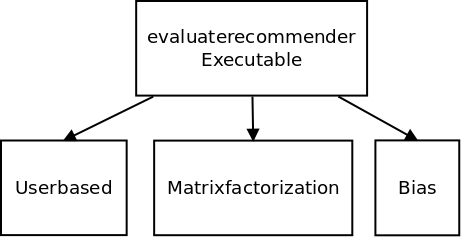
\includegraphics[width=0.5\textwidth]{structur}
  \caption{Projektstruktur}
  \label{fig:structur}
\end{figure}

\begin{description}
\item[evaluaterecommender] Dieses Modul enthält das ausführbare Programm. Es nutzt die Module Userbased, Matrixfactorisation und Bias um die Evaluation durchzuführen. Der Programmcode für die MAE Berechnung ist ebenfalls in diesem Modul enthalten.
\item[Userbased] Das Modul Userbased enthält den User-based CF Recommender.
\item[Matrixfactorization] Das Modul enthält einen Recommender der Matrixfaktorisierung nutzt.
\item[Bias] Das Modul Bias implementiert die unpersönlichen Empfehlungstechniken.
\end{description}

\subsection{Build System}
\label{sec:cabal}

Um das Projekt zu kompilieren und die Abhängigkeiten aufzulösen, wurde das Buildtool Cabal eingesetzt. Die verwendete Version ist 1.20.0.2. Cabal ist ein Paketisierung und Build System für Haskell. Cabal wird verwendet, weil die Implementierung der Algorithmen Pakete aus dem Repository Hackage verwendet. Cabal löst Abhängigkeiten zu Hackage Paketen automatisch auf. Ausserdem verwaltet Cabal Projektmetadaten wie Lizenz, Author, u.s.w.

\subsubsection{Sandboxing}
\label{sec:sanboxing}

Das Projekt wurde in einer sogenannten Sandbox erstellt. Wenn das Projekt in einer Sandbox erstellt wird, werden alle Abhängigkeiten des Projekts in einer separaten Paketverwaltung installiert. Das hat den Vorteil, dass Änderungen an der globalen Paketverwaltung das Projekt nicht beeinflussen. Der Befehl lautet:
\begin{verbatim}
cabal sandbox init
\end{verbatim}

\subsection{Daten einlesen}
\label{sec:readio}

Beim Einlesen der Daten sollte mit \verb|ByteString| gearbeitet werden. Dieser Abschnitt beschreibt, weshalb \verb|ByteString| eingesetzt wird.

Bei der Ausführung der Evaluation werden die Daten vom Filesystem eingelesen. Das Modul \verb|Prelude| bietet dafür die Funktion
\begin{verbatim}
readFile:: FilePath -> IO String
\end{verbatim}
 \verb|FilePath| ist ein Alias für \verb|String|. Die Funktion nimmt einen Dateipfad und gibt eine IO Action zurück. Die IO Action liest den Inhalt des Files und bindet Resultat an einen String.

Ein \verb|String| ist eine Liste. Listen werden in Haskell ``lazy'' evaluiert. Ein File ist für Haskell also nur eine Liste von Zeichen. Wenn die Listen lazy evaluiert werden sind die Elemente darin nur ein Versprechen, dass das Element zur Verfügung steht, wenn es benötigt wird. Die Berechnung des Elements hat noch nicht stattgefunden. Das ist normalerweise kein Problem aber wenn diese Liste ein Stream von der Festplatte ist, ist das Einlesen vergleichsweise langsam, weil jedes Zeichen einzeln von der Festplatte geholt wird.

Die Standardbibliothek Prelude bietet zwei Datentypen, die sich für das effiziente Einlesen der Daten eignen.

\begin{itemize}
\item \verb|Data.ByteString.Strict|
\item \verb|Data.ByteString.Lazy|
\end{itemize}

 Die Strict-Version löst das Problem indem der ganze String in den Arbeitsspeicher eingelesen wird. \verb|Data.ByteString.Lazy| liest die ersten 64KB in den Arbeitsspeicher \cite{Lipovaca}.

Da die Trainings und Testdaten ca. 1.7MB gross sind, wurde für dieses Projekt \verb|Data.ByteString.Strict| verwendet.

Listing \ref{lst:readio} zeigt wie Daten mit der Funktion \verb|readFile| eingelesen werden. Der ByteString wird der Funktion \verb|decode| übergeben. Diese gibt ein \verb|Either| zurück. Wenn ein Fehler beim Einlesen passiert enthält \verb|Either| eine Fehlermeldung. Sonst enthält es die gewünschten Daten. Ein möglicher Fehler wird in der Funktion \verb|toVec| abgefangen.

\begin{lstlisting}[label={lst:readio},caption={Einlesen von Files mit ByteString}]
import Data.Csv
import qualified Data.Vector as V
import qualified Data.ByteString.Lazy as Bl

type Rating = (Int, Int, Double)

main = do
  c <- Bl.readFile basefile
  let csvData = decode NoHeader c
  let v = toVec csvData
  ...

toVec :: Either String (V.Vector Rating)
      -> V.Vector Rating
toVec (Left err) = error err
toVec (Right v) = v
\end{lstlisting}

\subsection{Profiling}
\label{sec:profiling}

Die ersten Implementierungen der Collaborative Filtering Algorithmen haben oft zu viel Arbeitsspeicher alloziert und das Programm benötigte zu viel Zeit. Um Probleme der Skalierbarkeit zu lösen wurden Statistiken über das Verhalten der Algorithmen zur Laufzeit erstellt.

Der GHC Compiler unterstützt Time und Memory Profiling. Der generierte Output zeigt, wieviel Zeit und Speicher eine Funktion verursacht. Das heisst jede Funktion hat ein sogenanntes Kostencenter. Jedesmal wenn die Funktion aufgerufen wird, werden Zeit und Memory zu den vorhandenen Werten im Kostencenter hinzugezählt. Um die Werte im Kostencenter zu berechnen, generiert der Compiler zusätzlichen Code, der die Berechnung ausführt. Die zu analysierenden Programme müssen also mit der entsprechenden Compiler Option kompiliert werden \cite{Mena}.

Es können nur ausführbare Dateien analysiert werden. In diesem Projekt wurde das Programm \verb|evaluaterecommender| analysiert.

Um das Profiling einzuschalten, müssen drei Compiler Optionen gesetzt werden. Die Optionen können im Cabalfile im ghc-options Property gesetzt werden.
\begin{verbatim}
executable evaluaterecommender
  ghc-options:	-prof -fprof-auto -rtsopts
\end{verbatim}
\begin{description}
\item[-prof] Profiling wird eingeschaltet
\item[-fprof-auto] Zu jeder Funktion wird ein Kostencenter generiert.
\item[-rtsopts] Ermöglicht der Runtime Optionen mitzugeben
\end{description}

Alle verwendeten Pakete müssen mit der \verb|--enable-library-profiling|- Option kompiliert werden.

Um einen Profilingreport zu generieren, muss das Programm mit der Runtime Option \verb|-p| ausgeführt werden. Runtime Optionen können auf der Kommandozeile nach dem Programmnamen zwischen \verb|+RTS| und \verb|-RTS| mitgegeben werden.  

\begin{verbatim}
$ evaluaterecommender +RTS -p -RTS
\end{verbatim}

Das Programm generiert eine Textdatei \verb|evaluaterecommender.prof|. Diese teilt die Analyse in drei Teile auf.

Im obersten wird beschrieben, wie lange die Ausführung gedauert hat und wieviel Speicher konsumiert wurde. Im zweiten Teil werden die Funktionen, die am meisten Zeit und Speicher benötigen mit dem prozentualen Anteil aufgelistet. Im letzten Teil wird die Aufrufabfolge der Funktionen in Form eines Baumes beschrieben.

\begin{verbatim}
Wed Dec 24 15:05 2014 Time and Allocation Profiling Report 

evaluaterecommender +RTS -p -K100M -RTS

total time  =        0.74 secs   (741 ticks @ 1000 us,
total alloc = 1,259,391,232 bytes 

COST CENTRE   MODULE  %time %alloc

error            Main     34.7   52.3
updateRow2    Main     27.1   22.1
trainingcases Main      7.8    0.6
iter          Main      5.8    7.7
predict       Main      3.6    4.2

\end{verbatim}

\section{Fazit und Ausblick}
\label{sec:fazit}

Von den eigenen Implementierungen hat User-based CF den tiefsten durchschnittlichen Fehler bei der Evaluation erreicht. Im Gegensatz zu User-based CF ist Matrixfaktorisierung schwieriger zu implementieren und zu handhaben. Bei Matrixfaktorisierung mit Gradientenabstieg müssen 4 Parameter von Hand optimiert werden. Bei User-based CF muss nur die Nachbarschaftsgrösse $k$ optimiert werden.

Die Implementierung von Funks Gradientenabstiegverfahren hat sich als schwierig erwiesen. Da bei diesem Verfahren die Parametervektoren oft aktualisiert werden, wird viel Speicher alloziert und der Garbage Collector muss andauernd aufräumen. Deshalb ist es sinnvoll zu prüfen, ob das Optimierungsverfahren "`Funks stochastischer Gradientenabstieg"' nicht durch ein Verfahren ersetzt werden kann, dass einfacher zu parallelisieren ist. Da die verwendeten Datenstrukturen unveränderlich sind und die meisten Funktionen keinen Seiteneffekt haben, würde sich die Parallelisierung der Algorithmen anbieten.

Mit der Programmiersprache Haskell können die Recommender mit wenigen Zeilen Code implementiert werden. Das Package Repository Hackage bietet unter anderem Softwarebibliotheken für den Umgang mit Matrizen und Vektoren. Es enthält auch Statistikpakete, die für die Implementierung von Recommenender Systemen genutzt werden können.

\subsection{Implementierungsvergleich}
\label{sec:compare}

Die Implementierungen der beiden Algorithmen User-based CF und Matrixfaktorisierung wurden mit Implementierungen des LensKit Tools verglichen. 

LensKit ist eine Softwarebibliothek die verschiedene Recommender Algorithmen enthält. Sie wurde von GroupLens Research Lab Universität Minnesota \cite{ekstrandlk11} entwickelt. Sie eignet sich für den Vergleich, weil LensKit Implementierungen von User-based CF und Matrixfaktorisierung mit Funks SGD enthält.

Die LensKit Implementierungen wurden mit dem selben Datenset von MovieLens wie die beschriebenen Algorithmen evaluiert.

\begin{figure}
  \centering
\begin{tikzpicture}
\begin{axis}[
ybar,
enlargelimits=0.45,
legend style={at={(0.5,-0.15)},
anchor=north,legend columns=-1},
ylabel={MAE},
symbolic x coords={Userbased,Matrixfaktorisierung},
xtick=data,
ybar=5pt,% configures ‘bar shift’
bar width=9pt,
nodes near coords,
nodes near coords align={vertical},
]
\addplot coordinates {(Userbased,0.66) (Matrixfaktorisierung,0.74)}; 
\addplot coordinates {(Userbased,0.65) (Matrixfaktorisierung,0.63)};

\legend{eigene,LensKit}
\end{axis}
\end{tikzpicture} 
  
  \caption{Implementierungsvergleich mit LensKit}
  \label{fig:compareimpl}
\end{figure}

Die LensKit Implementierungen liefern in beiden Fällen einen tieferen MAE. LensKit zeigt, dass mit Matrixfaktorisierung die besten Resultate erreicht werden können. 

Bei der eigenen Implementierung des Recommenders mit Matrixfaktorisierung werden die User- und Itemtendenzen (siehe Abschnitt \ref{sec:simple}) nicht berücksichtigt. Gemäss \cite{koren2009} wird der mittlere Fehler durch die Berücksichtigung der Tendenzen minimiert. Die eigene Implementation kann also noch verbessert werden.

\section{Anhang}

\subsection{Euklidische Distanz}
\label{sec:euclid}

Der Pearson Korrelationkoeffizient ist nicht definiert, wenn die Varianz der betrachteten Bewertungen 0 ist. Deshalb wurde eine alternative Ähnlichkeitmetrik untersucht. \cite{segaran} schlägt vor die euklidische Distanzmetrik für User-based CF zu verwenden. Die euklidische Distanz ist auch definiert, wenn die Varianz 0 ist.

Jeder User wird als Vektor dargestellt. Die Bewertungen, die der User gemacht hat, sind die Elemente des Vektor. Die euklidische Distanz berechnet den geometrischen Abstand der Vektoren. Für zwei User $u$ und $v$ mit $n$ gemeinsamen Items, wird die euklidische Distanz $sim(u,v)$ wie folgt berechnet:

\begin{equation}
  \label{eq:euclid}
 sim(u,v) = \sum_i^n (u_i - v_i )^2
\end{equation}

Die euklidische Distanz berücksichtigt nicht, dass bestimmte User permanent höhere Wertungen geben.

\subsection{Hardware Plattform}
\label{platform}

Die Experimente wurden auf einem PC-Notebook durchgeführt. Das Notebook hat 8GB Ram und die CPU ist mit 2.9Ghz getaktet.

\begin{center}
\begin{tabular}{ll}
 Prozessor        &  i7-3520M            \\
 Clock            &  2.90GHz             \\
 Arbeitsspeicher  &  8 GB                \\
 Betriebssystem   &  Ubuntu 14.04.1 LTS  \\
\end{tabular}
\end{center}

\bibliographystyle{plain}
\bibliography{a}
\end{document}